\chapter*{About this project}
\paragraph{Abstract}
This project is intended to be an project that can be used in an educational 
environment. During the Data Structures and Algorithms module we had in 2nd year,
short videos were shown to us showing various sorting algorithms being 
visualized. It is a web-based application written in ReactJS, a web framework 
for building user interfaces. The project allows users to visualize various
sorting algorithms, which could be helpful in an educational context.
\par
\bigskip
This project also allows users to register and sign in to an account. From here, the user can record their screen and upload these sorts to a database. These sorts are available to be viewed by all users once logged in.

\chapter{Introduction}
This chapter serves as an introduction to the project. In it, the various aspects
of the project are discussed and the main objectives of the project. Each of the 
chapters are briefly discussed as well, detailing what each contains and what is
discussed in each.

\section{Discussion of the dissertation}
Throughout this dissertation, the following six chapters each covered a distinct aspect of the project:

\begin{itemize}
    \item \textbf{Chapter 1 - Introduction} - Chapter 1 serves as the introduction to the project, discussing the aim of the project, an overview of sorting algorithms, the project itself, the objectives of the project, and the scope of the project.
    \item \textbf{Chapter 2 - Methodology} - Chapter 2 covers the various research and software methodologies employed throughout, meetings with the project supervisor. development tools used, source control, and types of testing carried out.
    \item \textbf{Chapter 3 - Technology Review} - Chapter 3 introduces each of the different technologies, tools, and languages used to develop the project itself.
    \item \textbf{Chapter 4 - System Design} - Chapter 4 discusses the design of the system and goes over each of the main components of the application.
    \item \textbf{Chapter 5 - System Evaluation} - Chapter 5 evaluates the system as a whole, analysing the various aspects of the project and further discusses the type of testing carried out.
    \item \textbf{Chapter 6} - Chapter 6 serves as the conclusion to the project, evaluating the project further relative to initial objectives set out and testing.
\end{itemize}

\section{Aim of the project}
The aim of this project is to create a web-based application that allows users to
visualise various different sorting algorithms, allow user authentication and 
upload visualizations to a database from which other users can view and compare
the performance. This project is intended to be used in an educational sense,
providing an interactive application where user's can actively choose a sorting
algorithm to visualise, save these visualisations to view them at a later point.

\section{Sorting Algorithms}
In computer science, a sorting algorithm is an algorithm that rearranges 
elements of a list in a certain order, according to a comparison operator on the
elements. The comparison operator is used to decide the new order of element in the respective data structure. The most frequently used orders are numerical order and lexicographical order. Efficient sorting is important for optimizing the efficiency of other algorithms (such as search and merge algorithms) that require input data to be in sorted lists. Sorting is also often useful for canonicalizing data and for producing human-readable output. More formally, the output of any sorting algorithm must satisfy two conditions:

\begin{enumerate}
    \item The output is in non-decreasing order (each element is no smaller than 
    the previous element according to the desired total order)
    \item The output is a permutation (a reordering, yet retaining all of the 
    original elements) of the input
\end{enumerate}

Furthermore, the input data is often stored in an array, which allows random 
access, rather than a list, which only allows sequential access; though many 
algorithms can be applied to either type of data after suitable modification.

\section{Discussion of the project}
The project is sorting algorithm visualiser that allows users to choose a sorting
algorithm to visualise. It also supports user authentication, where users can 
register and sign-in to upload, save, and view previous sorts. The project came about from viewing
similar projects online and and an interest in finding out how such projects were
developed. The project also came about from developing something that could be 
used in an educational sense. In 2nd year of our course, we were enrolled in a 
Data Structures and Algorithms module from which we learned about various 
different algorithms, how they were performed, space time complexity, etc.

\newpage
\section{Objectives of the project}
There were several objectives I set out when first designing this project:

\begin{itemize}
    \item Create an application that can be used in an educational sense, which 
    can possibly be used for modules where students learn about data structures, 
    algorithms, space time complexity, etc.
    \item Create a web application that allows users to visualise several 
    different sorting algorithms.
    \item Allow users to register for an account and log in to save
    visualisations for later viewing.
    \item Allow user to upload previous sorts to viewing at a later point.
\end{itemize}

\section{Scope of the project}
\begin{center}
    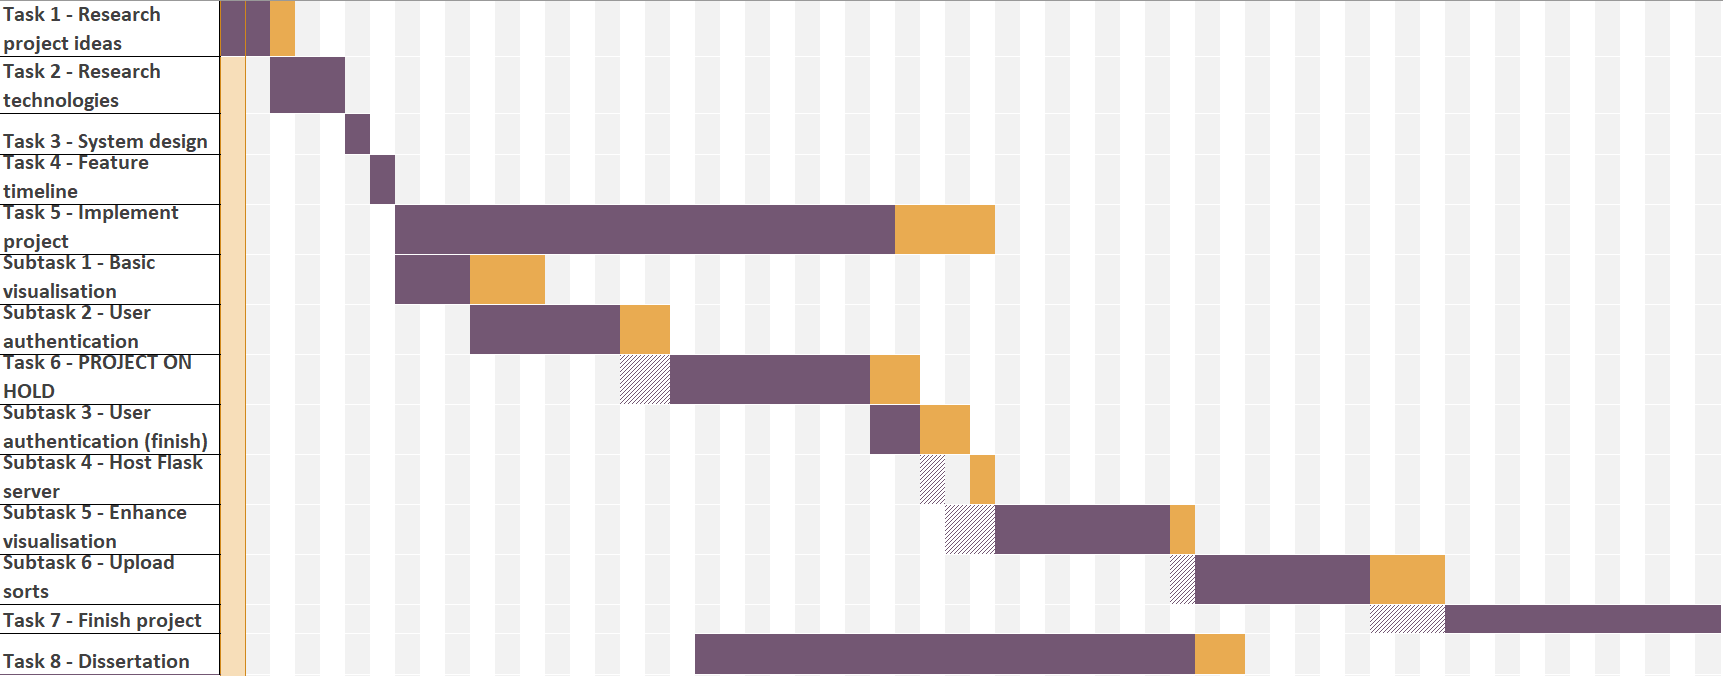
\includegraphics[scale=.3]{images/project_timeline} 
    \label{fig:project_timeline}
\end{center}
Above is the projected and actual timeline of the project. The first few weeks of the project comprised of different researching project ideas, evaluating each based on complexity and scope and, after the project idea was settled on, the next couple of weeks comprised of researching various technologies to see which would be the most suitable to develop the chosen project idea. After this, the system was designed, along with a timeline of approximately when each feature should be implemented and how long each should take. With all this complete, the actual development of the project was started. The first feature to be implemented was to get basic visualization working. With this done, user authentication was started, which included writing the relevant functions to allow a user to register and log in to an account. After Christmas the project was resumed and user authentication finished. The Flask server, containing the functionality to allow the user to register and log in, was hosted on PythonAnywhere. With this done, more algorithms were written and incorporated and the visualization were enhanced. The final steps of the project included enabling the user to record sorts and upload them, and hosting the project. 

\subsection{Project Requirements}
\begin{center}
    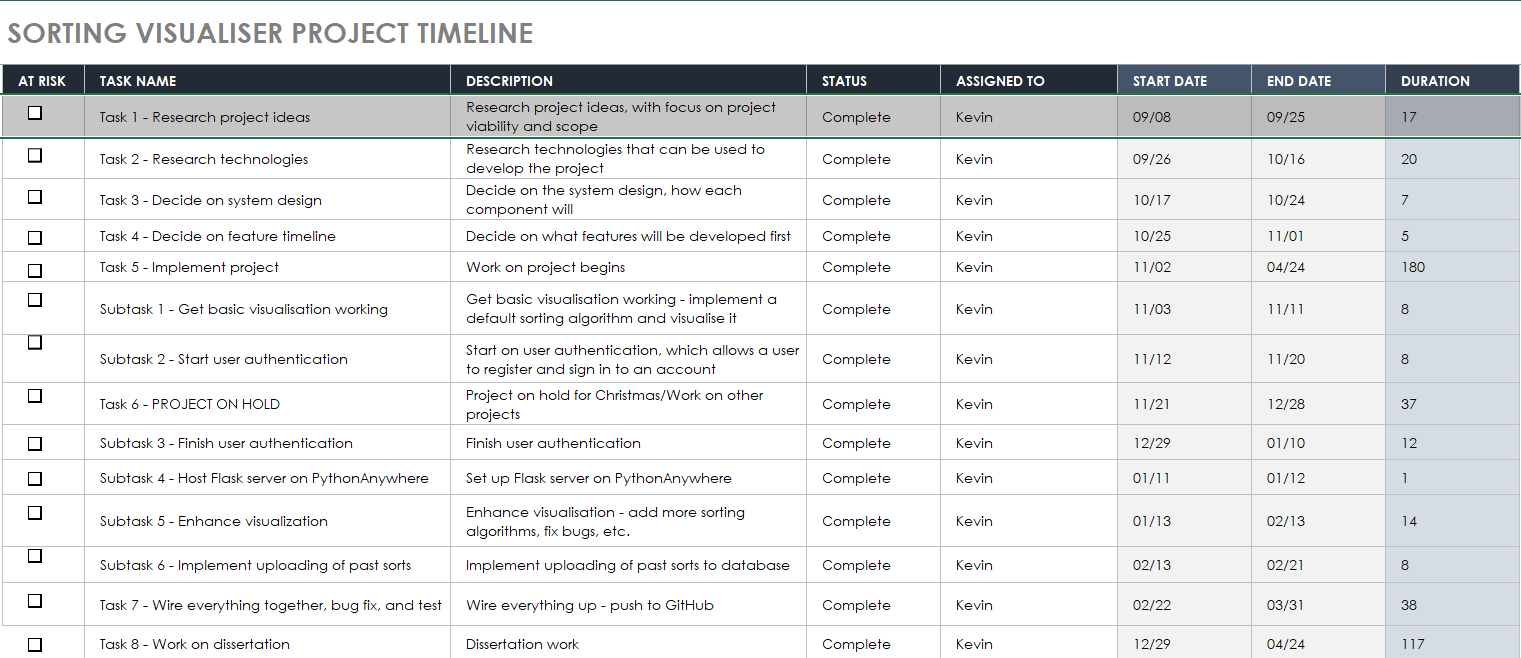
\includegraphics[width=16cm]{images/project_plan} 
    \label{fig:project_plan}
\end{center}
There were several project requirements that I set out when designing this
project. These can be seen in \ref{fig:project_timeline}. The functions and
features required were:

\begin{itemize}
    \item Visualisation of sorting algorithms
    \item Support of various sorting algorithms
    \item Upload of user created data sets
    \item User authentication
    \item Database support
\end{itemize}

\subsection{Project Limitations}
As a whole, the application is primarily built to sort elements represented in a
numerical format. The limitations of the project would be the inability to sort 
elements represented in a numerical format, special characters, files, etc. In the context of an algorithms visualiser, while being able to sort items like letters, special characters, files, etc. could very well be viable, visualising such things mightn't be as suitable as visualising the sorting of numbers.

\newpage
\subsection{Scope and context in relation to degree}
This project was about designing and implementing an application that could visualize various sorting algorithms, allow users to register and login to an account, record the sorts, upload previous sorts, and view these past sorts. This application is similar to several different applications already developed, such as the applications researched in Chapter 2, section 2.1. As such, the project related to the degree in several different areas. It contains a wide array of technologies and elements that were previously covered in the course. The elements contained in the application are databases, user authentication, data handling, data transfer, web front-end, and testing - much of which were covered in several modules throughout the course such as: 

\begin{itemize}
    \item \textbf{Data Structures and Algorithms}, which covered sorting algorithms - a major component of the application.
    \item \textbf{Software Testing}, which covered testing and greatly aided in making sure the application worked as intended and provided testing processes to thoroughly test the application.
    \item \textbf{Professional Practice in IT}, which first introduced to us undertaking a large project over a period of time and having a project supervisor to which we would meet with regularly to discuss the progress of the project.
    \item \textbf{Database Management Systems}, which primarily covered the use and integration of databases with applications.
\end{itemize}